

\begin{document}

\maketitle

\section{Introduction}

The High Energy Physics (HEP) \citep{HEP} -- often called Particle
Physics -- is one of the research areas where the accomplishment of
scientific results is  inconceivable without the infrastructure for
distributed computing, the Computing Grid. The HEP is a branch of
Physics that studies properties of elementary subatomic constituents
of matter. It goes beyond protons and neutrons to study particles
which existed only a fraction of a second after the Big Bang and
quarks and gluons in the so-called Quark Gluon Plasma (QGP) \cite{QGP}.
These studies are based on experiments with particles colliding at
very high energies, at speeds almost equal to the speed of light.

The world's leading Particle Physics research laboratory is CERN
\cite{CERN}, the European Center for Nuclear and Particle Physics near
Geneva, Switzerland. The CERN latest particle accelerator, the Large
Hadron Collider (LHC) \cite{LHC}, Figure 1, installed in a 27~km
long tunnel located about 100~m underground and crossing the Swiss -
French border, uses counter-rotating beams of protons or lead ions (Pb)
to collide at 4 points, inside large particle detectors: ALICE
\cite{ALICE}, ATLAS \cite{ATLAS}, CMS \cite{CMS} and LHCb \cite{LHCb}. There are also another two smaller
 experiments,  TOTEM \cite{TOTEM} and LHCf \cite{LHCf}. The later two are much smaller in size and they are designed
 to focus on forward particles, (particles that just brush past each other 
as the beams collide, rather than meeting head-on).

The energy of the protons is
currently 3.5~TeV (1 Tera eV= 1 million MeV) and that of the Pb ions is
1.38~TeV, so the collision energies are 7~TeV for the protons and
2.76~TeV for the Pb ions.

%fig01
\begin{figure}[htb] % h-here, t-top, b-bottom
\centering
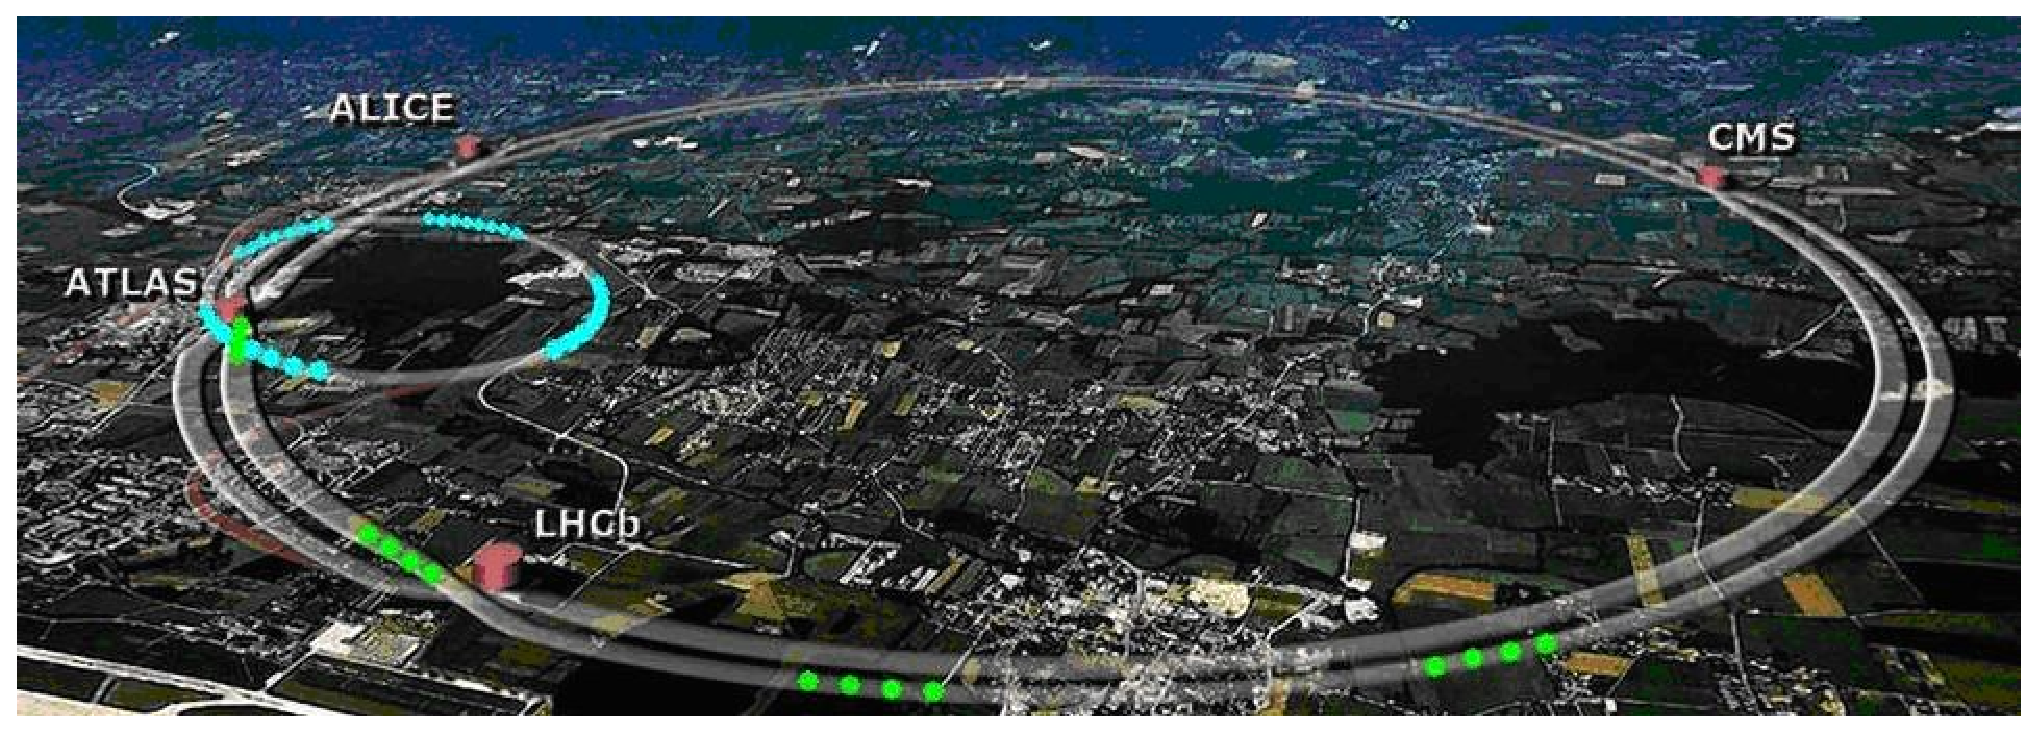
\includegraphics[width=13cm]{fig01.eps} %    ** if .eps don't need extension
\caption{LHC@CERN}\label{fig01}
\end{figure}



The phrase often used to summarize the mission of the LHC is, that
with the LHC we are going back in time very close to the Big Bang,
as close as about $10^{-10}$ seconds. In terms of length it represents
about $10^{-16}$ cm (compared to the dimensions of the Universe of about
$10^{28}$ cm). At this scale, the matter existed in a form of a ``soup''
made of the quarks and gluons, the Quark Gluon Plasma. The quarks
are objects protons and neutrons are made of, so the LHC represents
in a sense a huge extremely complicated microscope enabling the
study of the most basic elements of matter.

There are several major questions which scientists hope to
get answered with the help of the LHC:

\begin{itemize}
\item What is the origin of mass? Why do elementary particles have
some weight? And why do some particles have no mass at all? At
present, we have no established answers to these questions. The
theory offering a widely accepted explanation, the Standard Model
\cite{Standard}, assumes the existence of a so-called Higgs boson, a key particle
undiscovered so far, although it was first hypothesized in 1964. One
of the basic tasks of the LHC is to bring an established statement
concerning the existence of the Higgs boson.

\item Where did all the anti-matter disappear? We are living in the
World where everything is made of matter. We suppose that at the
start of the Universe, equal amounts of matter and antimatter were
produced in the Big Bang. But during the early stages of the
Universe, an un-known deviation or in-equilibrium must have happened
resulting in the fact that in our world today, hardly any antimatter
is left.

\item What are the basic properties of the Quark-Gluon Plasma, the
state of the matter existing for a tiny period of time after the Big
Bang? Originally, we thought it would behave like a plasma, but the
latest scientific results including those delivered by the LHC
suggest that it behaves like a perfect liquid,
which is somewhat surprising for us.

\item What is the universe made of? At the moment, the particles that we understand 
create only 4\% of the universe. The rest is believed to be made out of dark matter
and dark energy. The LHC experiments will look for supersymmetric particles, which
 would confirm a likely hypothesis for the creation of dark matter.
\end{itemize}

From the experiments analyzing the data from the LHC
collisions, ATLAS and CMS are the largest. They were nominally
designed to look for the Higgs boson but in fact these are general
purpose detectors for the study of all kinds of Physics phenomena at
the LHC  energy range. The
ALICE  detector is a dedicated heavy ions detector to study the
properties of the Quark Gluon Plasma formed in the collisions of
lead ions  at the LHC energies. The LHCb is much smaller detector and its
mission is to study the asymmetry between matter and antimatter. 
Although all these experiments are
designed for Particle Physics research, the scientific programs they
follow actually cross a border between Particle Physics,
Astrophysics and Cosmology.

Now, where does the Computing Grid show up in this scientific set-up?
The LHC is the world's largest particle accelerator. The protons and
lead ions are injected into the accelerator in bunches, in
counter-rotating beams. According to the original design proposal,
there should be 2808 bunches per a beam. Each bunch of protons
contains $10^{11}$ protons. the design beam energy is 7~TeV and the
design luminosity is $10^{34}\ $cm${}^{-2}$s${}^{-1}$. The bunch
crossing rate is 40~MegaHz and the proton collisions rate
$10^7-10^9$ Hz.

However, the new phenomena looked for by the scientists appear at a
rate of $10^{-5}$ Hz. So the physicists must analyze $10^{13}$
collision events/sec to have a chance to discover a New Physics
phenomenon. At present, the machine has not yet reached the full
number of bunches per beam and is operating at half of the
originally proposed energy, but the luminosity is getting rapidly to
the goal value. The LHC team has been increasing the number of
bunches gradually reaching 1380 bunches/beam at the time of writing.
The full beam energy will be reached in 2014, after one year of a
technical stop to arrange for this increase. The machine has already
beaten some world records which we will mention in section 5. Let us
just mention the one concerning the stored energy: in the end of
2010, the energy stored in the accelerator ring was about 28~MegaJoules (MJ).
At the target full intensity, this energy will
reach about 130~MJ which is an equivalent of 80~kg of TNT.

In any case, the volume of data necessary to analyze to discover New
Physics was already in the original proposal estimated to be about
15 PetaBytes (PB, 1PB=1 million GB) per data taking year. The number 
of the processor cores needed to process this
amount of data was estimated to be about 200 thousands. And here,
the concept of a distributed data management infrastructure comes
into the scenario, because there is no single computing
center within the LHC community/collaboration to offer such  massive
computing resources, even not CERN. Therefore in 2002, the concept
of the Worldwide LHC Computing Grid (WLCG) \cite{WLCG} was launched to
build a distributed computing infrastructure to provide the
production and analysis environments for the LHC experiments.

In the present chapter, we give a short overview of the Grid
computing for the experiments at the LHC and the basics of the
mission of the WLCG.  Since we are members of the ALICE
collaboration, we will also describe some specific features of the
ALICE distributed computing environment.

In section 2, we will describe the architecture of the WLCG, which
consist of an agreed set of services and applications running on the
Grid infrastructures provided by the WLCG partners. In section 3, we
will mention some of the middleware services provided by the WLCG
which are used for the data access, processing, transfer and
storage. Although WLCG depends on the underlying Internet - computer
and communications networks, it is the special kind of software, so-called
middleware, that enables the user to access computers
distributed over the network. It is called ``middleware'' because it
sits between the operating systems of the computers and the Physics
applications that solve particular problems. In section 4, the
Computing model of the ALICE experiment will be briefly described.
It provides guide lines for the implementation and deployment of the
ALICE software and computing infrastructure over the resources
within the ALICE Grid and includes estimates of the amount
of needed computing resources. Section 5
will be devoted to the ALICE-specific Grid services and the ALICE
Grid middleware AliEn. It is a set of tools and services which
represents an implementation of the ALICE distributed computing
environment integrated in the WLCG environment.  In section 6, an
overview will be given of the experience and performance of the WLCG
project and also of the ALICE Grid project in particular during the
real LHC data taking. The continuous operation of the LHC started in
November 2009.  When the data started to flow from the detectors,
the distributed data handling machinery was performing almost
flawlessly as a result of many years of a gradual development,
upgrades and stress-testing prior to the LHC startup. As a result of
the astounding performance of WLCG, a significant number of people
are doing analysis on the Grid, all the resources are being used up
to the limits and the scientific papers are produced with an
unprecedented speed within weeks after the data was recorded.

Section 7 contains a short summary and an outlook. This chapter is
meant to be a short overview of the facts concerning the Grid
computing for HEP experiments, in particular for the experiments at
the CERN LHC. The first one and half a year of the LHC operations
have shown that WLCG has built a true, well functioning distributed
infrastructure and the LHC experiments have used it to rapidly
deliver Physics results. The existing WLCG infrastructure has been
and will be continuously developing into the future absorbing and
giving rise to new technologies, like the advances in networking,
storage systems, middleware services and inter-operability between
Grids and Clouds.




